\documentclass[tikz, border=0.5cm]{standalone}
\usepgfmodule{nonlineartransformations} 
\usetikzlibrary{fpu}
\makeatletter
\newcommand{\PgfmathsetmacroFPU}[2]{\begingroup% https://tex.stackexchange.com/a/503835
\pgfkeys{/pgf/fpu,/pgf/fpu/output format=fixed}%
\pgfmathsetmacro{#1}{#2}%
\pgfmathsmuggle#1\endgroup}%
\def\conformaltransformation{% similar to the pgfmanual section 103.4.2
\PgfmathsetmacroFPU{\myphase}{atan2(\the\pgf@y,\the\pgf@x)}
\PgfmathsetmacroFPU{\myradius}{veclen(\pgf@y,\pgf@x)/1cm}
\PgfmathsetmacroFPU{\myx}{\myradius*\myradius*cos(2*\myphase)*0.2cm}%
\PgfmathsetmacroFPU{\myy}{\myradius*\myradius*sin(2*\myphase)*0.2cm}%
\pgf@x=\myx pt%
\pgf@y=\myy pt%
} 
\makeatother
\begin{document}

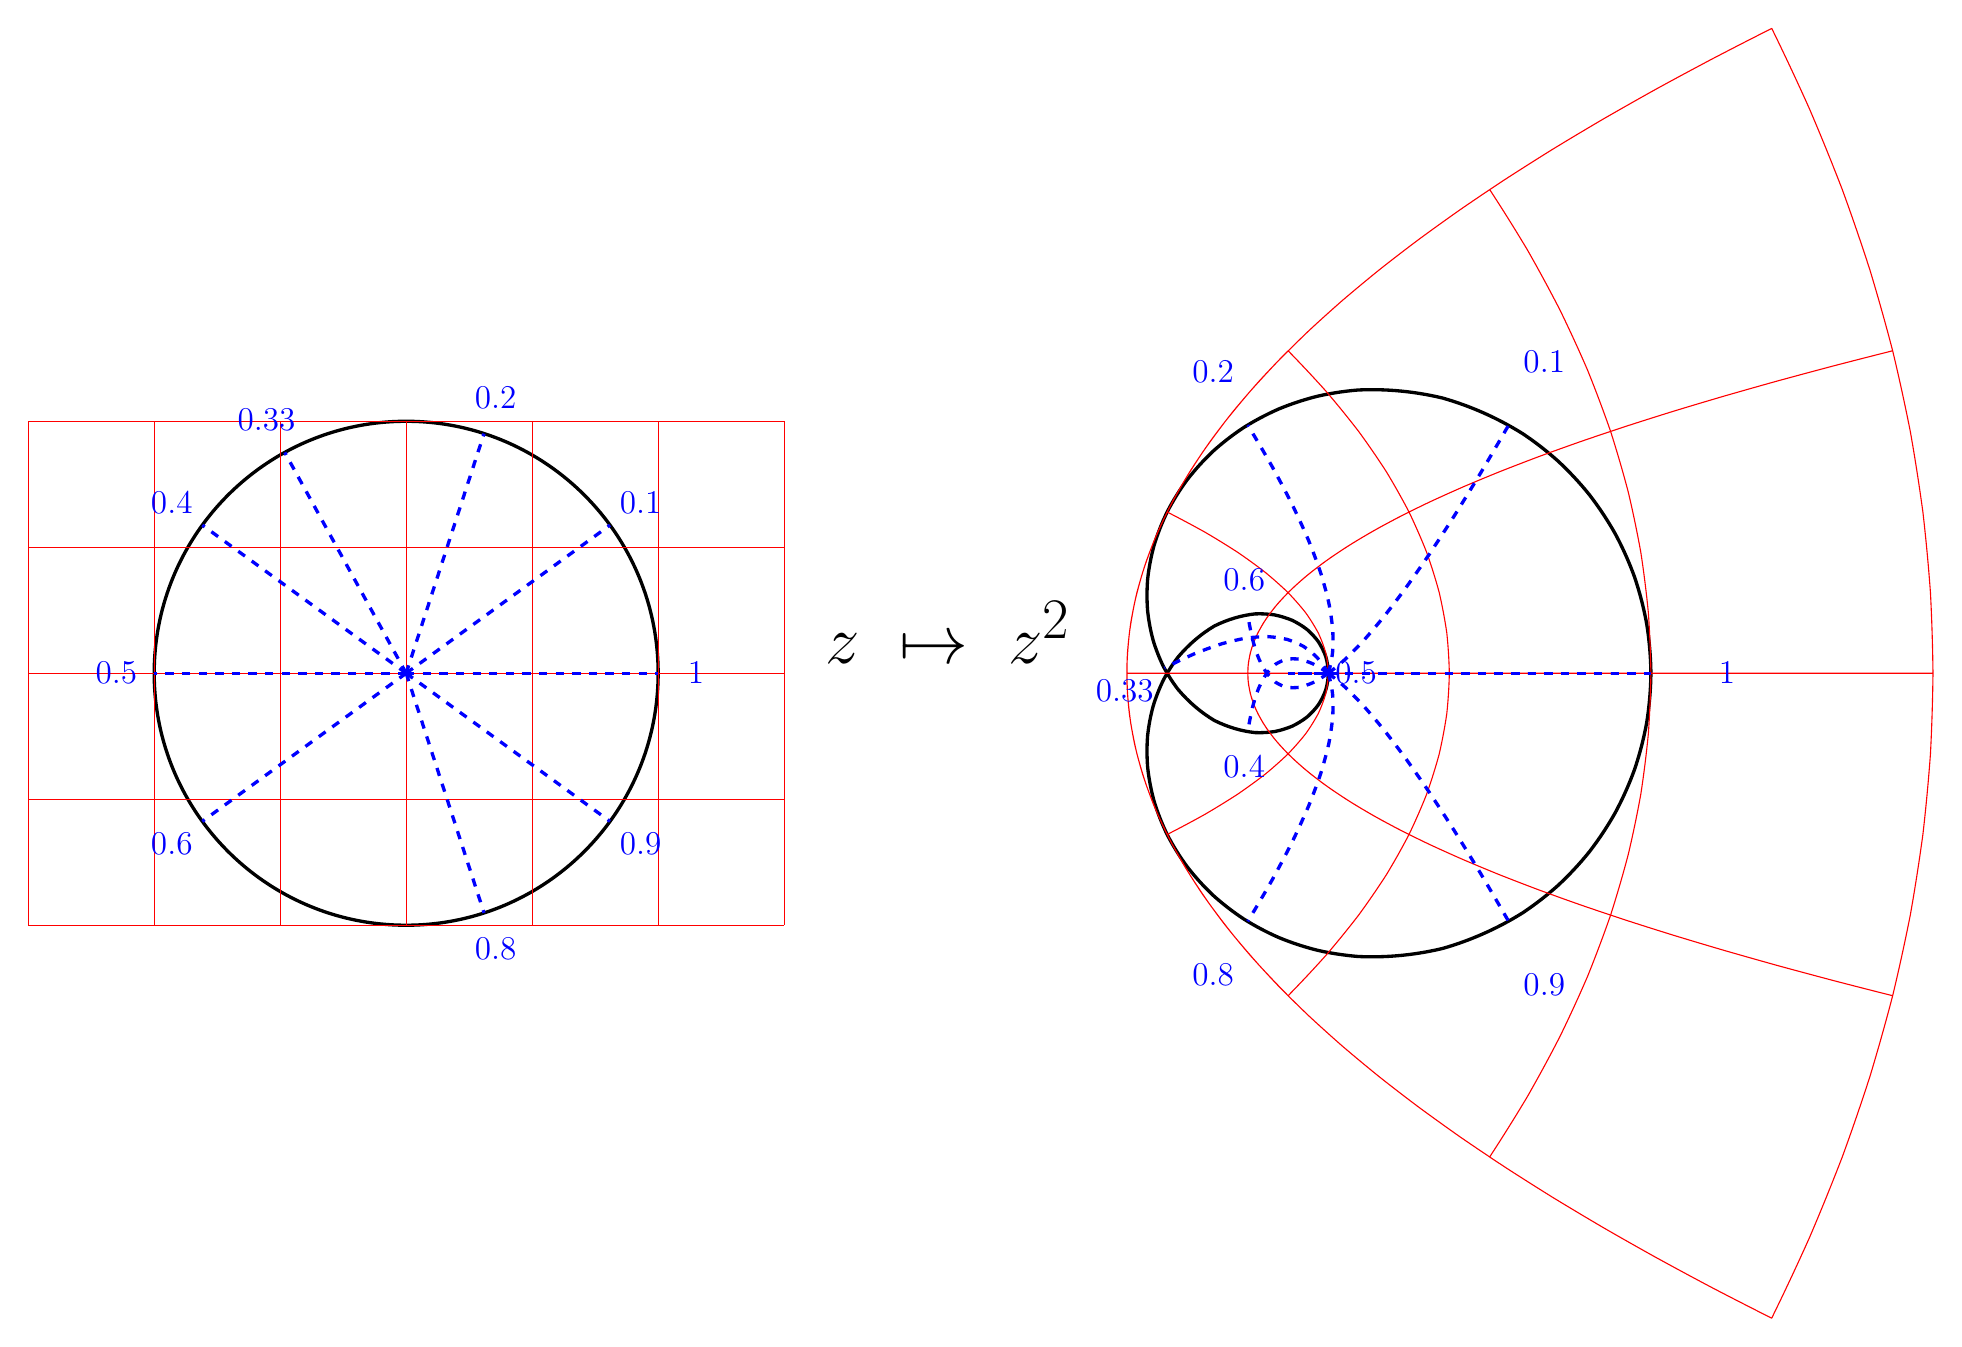
\begin{tikzpicture}[scale=1.6,font=\Huge]
\begin{scope}[xshift=-8cm]
    \draw[very thick, black] (1,0) circle(2);
    \draw[red] (-2,-2) grid (4,2);
    \foreach \n in {1.0,0.5,0.33,0.2,0.4,0.1,0.6,0.8,0.9} {
        \pgfmathsetmacro{\angle}{360 * \n}
        \draw[blue, dashed,very thick] (1,0) -- ({1+2*cos(\angle)}, {2*sin(\angle)});
        \node[blue,very thick] at ({1+2.3*cos(\angle)}, {2.3*sin(\angle)}) {\large\bfseries $\pgfmathprintnumber[fixed]{\n}$};
    }
    \node[above] at (5.3,0) {$z~\mapsto~z^2$};)
\end{scope} 
\begin{scope}
    \pgftransformnonlinear{\conformaltransformation}
    \draw[very thick, black] (1,0) circle(2);
    \draw[red] (-2,-2) grid (4,2);

    \foreach \n in {1.0,0.5,0.33,0.2,0.4,0.1,0.6,0.8,0.9} {
        \pgfmathsetmacro{\angle}{360 * \n}
        \draw[blue, dashed,very thick] (1,0) -- ({1+2*cos(\angle)}, {2*sin(\angle)});
        \node[blue,very thick] at ({1+2.3*cos(\angle)}, {2.3*sin(\angle)}) {\large\bfseries $\pgfmathprintnumber[fixed]{\n}$};
    }
\end{scope} 
\end{tikzpicture}
\end{document}
